\documentclass[12pt]{article}
\usepackage[brazil]{babel}
\usepackage[utf8]{inputenc}
\usepackage{amsmath}
\usepackage{amsfonts}
\usepackage{amssymb}
\usepackage{geometry}
\usepackage{graphicx}
\usepackage{float}
\usepackage{enumitem}
\usepackage{multicol}
\usepackage{array}
\usepackage{xcolor}


\newif\ifmostravermelho
\mostravermelhofalse %começa falso

\newcommand{\vermelho}[1]{%
  \ifmostravermelho
    {\color{red}#1}%
  \else
    #1%
  \fi
}

%\newcommand{\vermelho}[1]{{\color{red}#1}}
\geometry{a4paper, margin=1.2cm}
\setlength{\parindent}{1.2cm}

% Definindo o contador e o comando de questão
\newcounter{questao}
\newcommand{\novaquestao}[1]{%
  \stepcounter{questao}%
  \subsection*{Questão \thequestao\ (#1)}%
}

\title{ATIVIDADE AVALIATIVA DE MATEMÁTICA}
\author{CETI BILÍNGUE GILBERTO MESTRINHO DE MEDEIROS RAPOSO}
\date{}

\begin{document}
    % Cabeçalho reduzido
    \vspace{0.5cm}
    \begin{center}
        \large
        \begin{tabular}{|l l|}
            \hline
            \textbf{ESCOLA:} & EETI GILBERTO MESTRINHO DE MEDEIROS RAPOSO \\ 
            \textbf{ALUNA(O):} & \underline{\hspace{7cm}} \textbf{SÉRIE:} \underline{\hspace{1.5cm}} \textbf{TURMA:} \underline{\hspace{1.5cm}} \\
            \textbf{PROFESSOR:} & \underline{\hspace{7cm}} \textbf{DATA:} \underline{\hspace{1.5cm}}/\underline{\hspace{1.5cm}}/\underline{\hspace{1.5cm}} \\
            \textbf{VALOR:} & \underline{\hspace{3cm}} \textbf{NOTA:} \underline{\hspace{1.5cm}} \\
            \hline
        \end{tabular}
    \end{center}
    \vspace{0.5cm}
    
    % Título manual
    \begin{center}
        \Large\textbf{LISTA DE EXERCÍCIOS SOBRE GEOMETRIA ESPACIAL}
    \end{center}
    
    \vspace{0.3cm}
    
    \section*{\vermelho{ATENÇÃO:}}
    \begin{itemize}[noitemsep]
        \item Resolva toda a lista, justificando cada questão.
        \item Colocar o nome completo e identificação no cabeçalho.
        \item Faça na lista, se e somente se a resolução de cada questão couber em cada questão.
        \item Há apenas uma opção correta em cada questão de múltipla escolha.
        \item Caso opte por fazer numa folha à parte, identifique cada questão.
    \end{itemize}
    % Início das colunas com linha vertical

    \section*{Questões}
    \mostravermelhotrue
    \begin{multicols}{2}
        \columnseprule=0.4pt
        \columnsep=20pt
        
        \novaquestao{PSC-UFAM 2014}
            A figura a seguir é composta por uma pirâmide hexagonal regular inscrita em um prisma hexagonal regular reto. Podemos afirmar que:

            \begin{center}
                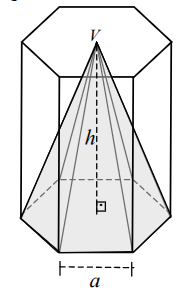
\includegraphics[scale=0.6]{q3.png}
            \end{center}
        
            \begin{enumerate}[label=(\Alph*), noitemsep]
                \item \vermelho{O volume da pirâmide é um terço do volume do prisma.} %
                \item O volume do prisma é o dobro do volume da pirâmide.
                \item A área total da pirâmide é um terço da área total do prisma.
                \item A área total do prisma é um terço da área total da pirâmide.
                \item A área lateral da pirâmide é um terço da área total do prisma.
            \end{enumerate}
        
        \novaquestao{PSC-UFAM 2014}
            Um reservatório possui a forma de um paralelepípedo reto retângulo, conforme a figura a seguir:

            \begin{center}
                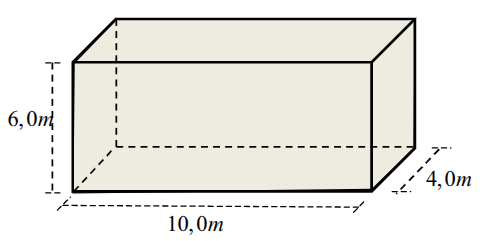
\includegraphics[scale=0.6]{q4.png}
            \end{center} Admitindo que 1 litro equivale a $1 \ dm^{3}$ , para que o tanque esteja completamente cheio são necessários:
        
            \begin{enumerate}[label=(\Alph*), noitemsep]
                \item $2,4 \times 10^{7}$ litros
                \item \vermelho{$2,4 \times 10^{5}$ litros} %
                \item $2,4 \times 10^{6}$ litros
                \item $2,4 \times 10^{4}$ litros
                \item $2,4 \times 10^{-4}$ litros
            \end{enumerate}
        
        \novaquestao{PSC - UFAM 2017}
            Numa região distante de determinada cidade, deseja-se construir um reservatório com a forma de um tronco de pirâmide hexagonal regular. Para atender às necessidades do lugar e às restrições orçamentárias, a altura do tronco da pirâmide deve ser de 8 m e as arestas das bases devem medir 4 m e 6 m. O volume (em $m^{3}$ desse reservatório será, aproximadamente: (Observação: use $\sqrt{3} = 1,7)$ \\

            \begin{center}
                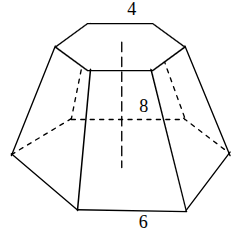
\includegraphics[scale=0.6]{q8.png}
            \end{center}
            \begin{enumerate}[label=(\Alph*), noitemsep]
                \item 114,1
                \item 343,5
                \item 482,7
                \item \vermelho{516,8}  %
                \item 892,0
            \end{enumerate}
        
        \novaquestao{PSC-UFAM 2017 / Adaptada}
            Desenvolvendo a superfície lateral de um cone circular reto, obtém-se um setor circular de raio 8 cm e ângulo central $135^\circ$. O volume (em $cm^{3}$) e a área total (em $cm^{2})$ do cone devem ser, respectivamente:

            \begin{center}
                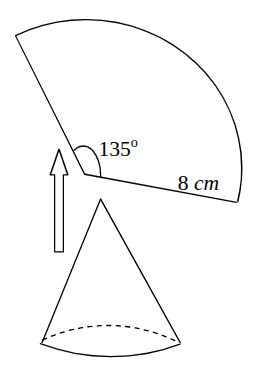
\includegraphics[scale=0.6]{q10.png}
            \end{center}
        
            \begin{enumerate}[label=(\Alph*), noitemsep]
                \item $3\pi$ e $53\pi$
                \item $9\pi\sqrt{45}$ e $23\pi$
                \item \vermelho{$3\pi\sqrt{55}$ e $33\pi$} %
                \item $3\pi\sqrt{65}$ e $43\pi$
                \item $3\pi\sqrt{75}$ e $66\pi$
            \end{enumerate}
        
        \novaquestao{PSC-UFAM 2018}
            Na figura a seguir, o volume do sólido com vértices nos pontos A, D, E, H, G é, em $cm^{3}$:

            \begin{center}
                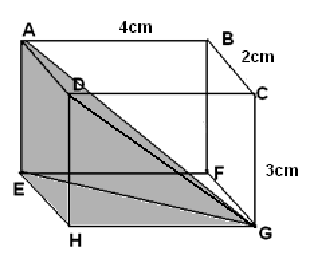
\includegraphics[scale=0.6]{q11.png}
            \end{center}
            
            \begin{enumerate}[label=(\Alph*), noitemsep]
                \item ${8}/{3}$
                \item 6
                \item \vermelho{8} %
                \item 12
                \item 24
            \end{enumerate}
        
        \novaquestao{PSC-UFAM 2019}
            Sobre um tetraedro regular de aresta medindo 6 cm, é \textbf{CORRETO} afirmar que:
        
            \begin{enumerate}[label=(\Alph*), noitemsep]
                \item \vermelho{Seu volume é igual a $18\sqrt{2}\ cm^{3}$} %
                \item Sua altura mede $3\sqrt{6}\ cm$
                \item O apótema da base mede $2\sqrt{3}\ cm$
                \item Sua área lateral é igual a $27\sqrt{2}\ cm^{2}$
                \item Sua área total é igual a $36\sqrt{6}\ cm^{2}$
            \end{enumerate}
        
        \novaquestao{PSC-UFAM 2020}
            Uma loja de perfumaria vende alguns perfumes com formato de sólidos geométricos. O perfume de 50 ml mais vendido na loja tem o formato conforme indicado na figura a seguir:
            
            \begin{center}
                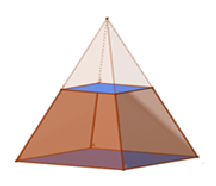
\includegraphics[scale=0.6]{q13.png}
            \end{center} Este frasco é uma pirâmide de base quadrada, cujo lado da base maior mede $5\ cm$ e o lado da base menor mede $2\ cm$. Se a altura das faces laterais da tampa mede $\sqrt{2}\ cm$ , qual deve ser a altura, em cm, de uma caixa que cobre todo este perfume?
        
            \begin{enumerate}[label=(\Alph*), noitemsep]
                \item Menor que {63}/{13}
                \item \vermelho{Maior que {63}/{13}} %
                \item Maior ou igual a {51}/{13}
                \item Maior que {50}/{13}
                \item Maior que {50}/{13} e menor que {63}/{13}
            \end{enumerate}
        
        \novaquestao{PSC-UFAM 2021}
            Aumentando em $2\ cm$ a aresta de um cubo, sua área total aumenta em $384\ cm^{2}$. Logo, o volume do cubo original era igual a: 
        
            \begin{enumerate}[label=(\Alph*), noitemsep]
                \item $1854\ cm^{3}$
                \item $2172\ cm^{3}$
                \item $2856\ cm^{3}$
                \item \vermelho{$3375\ cm^{3}$} %
                \item $4220\ cm^{3}$
            \end{enumerate}
        
        \novaquestao{PSC-UFAM 2022}
            Dois recipientes, um cilíndrico e um cônico, têm a mesma altura e bases com raios iguais. Se a capacidade do recipiente cônico é de 205 mL, então a capacidade do recipiente cilíndrico é de:
        
            \begin{enumerate}[label=(\Alph*), noitemsep]
                \item $205\ ml$
                \item $410\ ml$
                \item $505\ ml$
                \item \vermelho{$615\ ml$} %
                \item $750\ ml$
            \end{enumerate}
        
        \novaquestao{PSC-UFAM 2022}
            Uma fábrica armazena seus produtos em caixas de papelão com forma de prisma reto, cujas medidas estão indicadas na figura a seguir:

            \begin{center}
                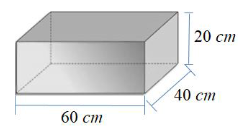
\includegraphics[scale=0.6]{q16.png}
            \end{center} Considerando que em certa semana foram usadas 10.000 dessas caixas e, desconsiderando os desperdícios, podemos afirmar que foram utilizados para confeccionar todas as caixas:
        
            \begin{enumerate}[label=(\Alph*), noitemsep]
                \item $4.400\ m^{2}$ de papelão
                \item $5.900\ m^{2}$ de papelão
                \item $6.200\ m^{2}$ de papelão
                \item $7.400\ m^{2}$ de papelão
                \item \vermelho{$8.800\ m^{2}$ de papelão}%
            \end{enumerate}
        
        \novaquestao{PSC-UFAM 2023}
            Uma piscina tem $10\ m$ de comprimento, $8\ m$ de largura e $1,8\ m$ de profundidade. O volume, em litros, dessa piscina é:
        
            \begin{enumerate}[label=(\Alph*), noitemsep]
                \item 110000
                \item 115000
                \item 125000
                \item 132000
                \item \vermelho{144000} %
            \end{enumerate}
        
        \novaquestao{PSC-UFAM 2023}
            Uma pirâmide regular, de base quadrada, possui área da base igual a $50\ dm^{2}$. Sabendo que o apótema da pirâmide mede $6\ dm$, podemos afirmar que a altura dessa pirâmide mede:        
        
            \begin{enumerate}[label=\alph*), noitemsep]
                \item \vermelho{$\sqrt{23,5}\ dm$} %
                \item $\sqrt{32,5}\ dm$
                \item $\sqrt{42,5}\ dm$
                \item $\sqrt{53,5}\ dm$
                \item $\sqrt{64,5}\ dm$
            \end{enumerate}
        
        \novaquestao{PSC-UFAM 2023}
            Um cilindro reto possui área total igual a $32\pi\ cm^{2}$. Sabendo que o raio da base é {1}/{3} da medida da altura desse cilindro, então a área lateral desse cilindro mede:
        
            \begin{enumerate}[label=(\alph*), noitemsep]
                \item $12\pi\ cm^{2}$
                \item $18\pi\ cm^{2}$
                \item $20\pi\ cm^{2}$
                \item \vermelho{$24\pi\ cm^{2}$} %
                \item $28\pi\ cm^{2}$
            \end{enumerate}

        \novaquestao{SIS - UEA 2019}
            Um prisma reto, de 8 cm de altura, tem como base um polígono de seis lados, conforme mostra a figura.
            
            \begin{center}
                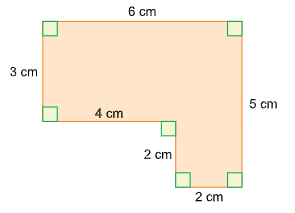
\includegraphics[scale=0.6]{q7.png}
            \end{center} O volume desse prisma é:
        
            \begin{enumerate}[label=(\Alph*), noitemsep]
                \item $160 \ cm^{3}$
                \item $168 \ cm^{3}$
                \item \vermelho{$176 \ cm^{3}$} %
                \item $184 \ cm^{3}$
                \item $192 \ cm^{3}$
            \end{enumerate}

        \novaquestao{SIS-UEA 2022}
            Considere um sólido oco, com a forma de paralelepípedo reto-retângulo, contendo $1 344\  cm^{3}$ de água, com faces e arestas de espessura desprezível, em que uma das arestas mede $16\ cm$ e outra aresta mede $12\ cm$. Esse sólido está apoiado sobre uma das faces de maneira que a altura da coluna de água seja igual a $14\ cm$. A área total desse sólido é:
        
            \begin{enumerate}[label=(\alph*), noitemsep]
                \item $800\ cm^{2}$
                \item \vermelho{$832\ cm^{2}$} %
                \item $864\ cm^{2}$
                \item $896\ cm^{2}$
                \item $928\ cm^{2}$
            \end{enumerate}

        \novaquestao{SIS-UEA 2023}
            Um prisma reto tem por base um pentágono com dois ângulos retos, conforme mostra a figura 1.

            \begin{center}
                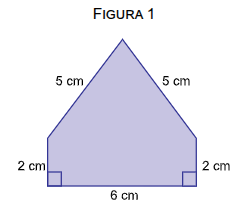
\includegraphics[scale=0.6]{q1-fig1.png}
            \end{center} O volume desse prisma é igual a $168\ cm^{3}$ e a figura 2 mostra uma vista desse prisma quando está apoiado sobre um dos pentágonos.

            \begin{center}
                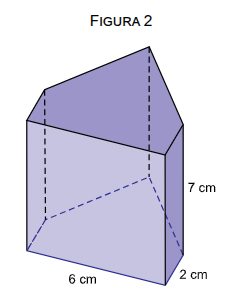
\includegraphics[scale=0.6]{q1-fig2.png} 
            \end{center} A área total desse prisma, em $cm^{2}$, é:
        
            \begin{enumerate}[label=(\alph*), noitemsep]
                \item 140
                \item 164
                \item \vermelho{188} %
                \item 212
                \item 236
            \end{enumerate}

        \novaquestao{SIS-UEA 2023}
            Em um cilindro reto, sua secção transversal é um círculo de raio $6\ cm$ e sua secção meridiana é um retângulo de área $96\ cm^{2}$ .

            \begin{center}
                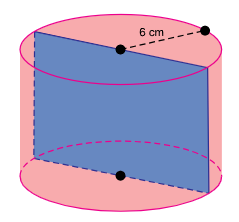
\includegraphics[scale=0.6]{q22.png}
            \end{center} A altura desse cilindro é:
            \begin{enumerate}[label=(\alph*), noitemsep]
                \item $6\pi\ cm$
                \item $16\pi\ cm$
                \item $4\pi\ cm$
                \item \vermelho{$8\ cm$} %
                \item $6\ cm$
            \end{enumerate}

        \novaquestao{SIS-UEA 2024}
            Uma das faces de um paralelepípedo retorretângulo tem $44\ cm^{2}$ de área, sendo que nessa face a medida da maior aresta excede a medida da menor aresta em $7\ cm$. Sabendo que o volume desse paralelepípedo é $308\ cm^{3}$ , sua área total é:

            \begin{enumerate}[label=(\alph*), noitemsep]
                \item \vermelho{$298\ cm^{2}$} %
                \item $336\ cm^{2}$
                \item $352\ cm^{2}$
                \item $412\ cm^{2}$
                \item $448\ cm^{2}$
            \end{enumerate}

        \novaquestao{SIS-UEA 2015}
            Determinado tipo de giz de lousa tem a forma de um prisma reto de base quadrada envolvido parcialmente em papel, e é vendido em caixas com 12 unidades, conforme mostra a figura e o esquema matemático.
        
            \begin{center}
                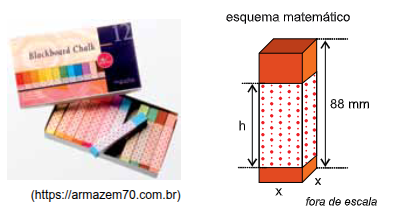
\includegraphics[scale=0.6]{q4-sis.png}
            \end{center} Sabendo que o volume de um giz é $12,672 \ cm^{3}$ e que a altura h do papel que o envolve corresponde a $3/4$ da altura do giz, é correto concluir que a quantidade aproximada de papel, em $cm^{2}$ necessária para recobrir os 12 gizes da
            caixa é:
        
            \begin{enumerate}[label=(\Alph*), noitemsep]
                \item 320
                \item 340
                \item 360
                \item \vermelho{380} %
                \item 400
            \end{enumerate}

        \novaquestao{MACRO-UEA 2024}
            Uma fábrica de doces faz bombons maciços de chocolate na forma de um prisma reto de base quadrada e com $1,5\ cm$ de altura, conforme mostra a figura.

            \begin{center}
                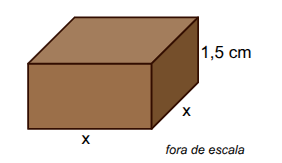
\includegraphics[scale=0.6]{q24.png}
            \end{center} Sabendo que para fabricar 85 bombons desse tipo são necessários $510\ cm^{3}$ de massa de chocolate, a medida da aresta da base, indicada na figura pela letra x, é igual a
        
            \begin{enumerate}[label=(\alph*), noitemsep]
                \item 1,5  cm
                \item 0,5  cm
                \item 2,5  cm
                \item 1,0  cm
                \item \vermelho{2,0  cm} %
            \end{enumerate}

        \novaquestao{MACRO-UEA 2023}
            Em uma caneca, no formato de um cubo com arestas internas medindo 7 cm, foram colocados 245 mL de café, que não preencheram totalmente a caneca, restando ainda um espaço entre a superfície do café e a borda superior da caneca, conforme figura.

            \begin{center}
                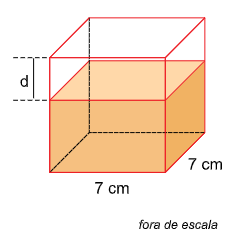
\includegraphics[scale=0.6]{q28.png}
            \end{center} A distância entre a altura do café, no interior da caneca, e a borda superior da caneca, indicada na figura pela letra d, é igual a:
        
            \begin{enumerate}[label=(\alph*), noitemsep]
                \item 3  cm
                \item 4  cm
                \item \vermelho{2  cm} %
                \item 5  cm
                \item 1  cm %
            \end{enumerate}

            \novaquestao{MACRO-UEA (Exatas) 2024}

                Um sólido, no formato de um cilindro circular reto, tem volume igual a $54\pi\ cm^{3}$, e sua área lateral $(A_{L})$ é calculada pela expressão $A_{L}=2\pi \times R \times H$, em que R e H são, respectivamente, o raio da base e a altura do cilindro. Sabendo que a medida da altura desse cilindro é o dobro da medida do raio da sua base, a área lateral desse cilindro, em $cm^{2}$, é:
            
                \begin{enumerate}[label=(\alph*), noitemsep]
                    \item \vermelho{$36\pi$}
                    \item $27\pi$
                    \item $32\pi$
                    \item $40\pi$
                    \item $42\pi$
                \end{enumerate}

        \novaquestao{ENEM 2023}
            Uma indústria de sucos utiliza uma embalagem no formato de prisma reto de base quadrada, com aresta da base de medida a e altura de medida h, ambas de mesma unidade de medida, como representado na figura.
            
            \begin{center}
                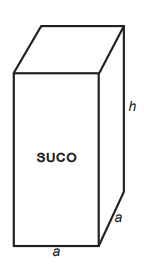
\includegraphics[scale=0.6]{q5.png}
            \end{center} Deseja-se criar uma linha de produção para uma nova embalagem de igual formato, mas que deverá ter uma capacidade igual ao triplo da atual. A altura da nova embalagem será igual a {4}/{3} da altura da embalagem atual. As arestas da base da nova embalagem serão denominadas de x. 
            Qual a relação de dependência entre a medida x da nova aresta da base e a medida a da aresta atual?
        
            \begin{enumerate}[label=(\Alph*), noitemsep]
                \item $x = a$
                \item $x = 3a$
                \item $x = 9a$
                \item \vermelho{$x = 3a / 2$} %
                \item $x = a\sqrt{3}$
            \end{enumerate}

        \novaquestao{ENEM 2021}

            Num octaedro regular, duas faces são consideradas opostas quando não têm nem arestas, nem vértices em comum. Na figura, observa-se um octaedro regular e uma de suas planificações, na qual há uma face colorida na cor cinza escuro e outras quatro faces numeradas.

            \begin{center}
                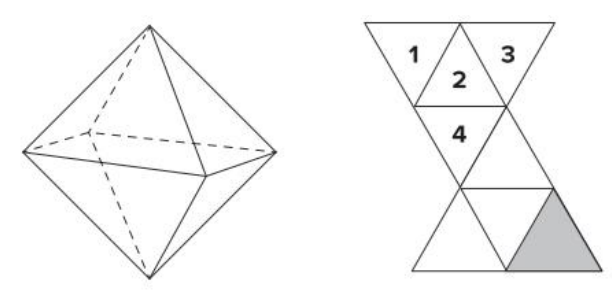
\includegraphics[scale=0.4]{q23.png}
            \end{center} Qual(is) face(s) ficará(ão) oposta(s) à face de cor cinza escuro, quando o octaedro for reconstruído a partir da planificação dada?
        
            \begin{enumerate}[label=(\alph*), noitemsep]
                \item 1, 2, 3 e 4
                \item 1 e 3
                \item 1
                \item 2
                \item \vermelho{4} %
            \end{enumerate}

        \novaquestao{ENEM 2010}
            Uma fábrica produz barras de chocolates no formato de paralelepípedos e de cubos, com o mesmo volume. As arestas da barra de chocolate no formato de paralelepípedo medem 3cm de largura, 18cm de comprimento e 4cm de espessura. Analisando as características da figuras geométricas descritas, a medida das arestas dos chocolates que têm o formato de cubo é igual a:
            
            \begin{enumerate}[label=(\alph*), noitemsep]
                \item 5  cm
                \item \vermelho{6  cm} %
                \item 12  cm
                \item 24  cm
                \item 25  cm 
            \end{enumerate}

        \novaquestao{ENEM 2010}
            Um arquiteto está fazendo um projeto de iluminação de ambiente e necessita saber a altura que deverá instalar a luminária ilustrada na figura.

            \begin{center}
                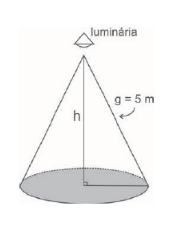
\includegraphics[scale=0.6]{q30.png}
            \end{center} Sabendo-se que a luminária deverá iluminar uma área circular de $28,26\ m^{2}$, considerando $\pi \approx 3,14$, a altura h será igual a:
        
            \begin{enumerate}[label=(\alph*), noitemsep]
                \item 3  cm
                \item \vermelho{4  cm} %
                \item 5  cm
                \item 9  cm
                \item 16  cm 
            \end{enumerate}

        \novaquestao{ENEM 2010}
            Dona Maria, diarista na casa da família Teixeira, precisa fazer café para servir as vinte pessoas que se encontram numa reunião na sala. Para fazer o café, Dona Maria dispõe de uma leiteira cilíndrica e copinhos plásticos, também cilíndricos.

            \begin{center}
                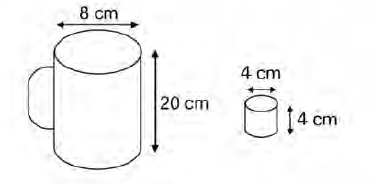
\includegraphics[scale=0.6]{q31.png}
            \end{center} Com o objetivo de não desperdiçar café, a diarista deseja colocar a quantidade mínima de água na leiteira para encher os vinte copinhos pela metade. Para que isso ocorra, Dona Maria deverá:

            \begin{enumerate}[label=(\alph*), noitemsep]
                \item \vermelho{Encher a leiteira até a metade, pois ela tem um volume 20 vezes maior que o volume do copo.} \\ %
                \item Encher a leiteira toda de água, pois ela tem um volume 20 vezes maior que o volume do copo. \\
                \item Encher a leiteira toda de água, pois ela tem um volume 10 vezes maior que o volume do copo. \\
                \item Encher duas leiteiras de água, pois ela tem um volume 10 vezes maior que o volume do copo. \\
                \item Encher cinco leiteiras de água, pois ela tem um volume 10 vezes maior que o volume do copo. 
            \end{enumerate}
        

        \novaquestao{EEAR-SP 2022}
            Seja um prisma reto de 15 cm de altura. Suas bases são trapézios de 6 cm e 4 cm de base e 5 cm de altura. O volume deste prisma equivale a $ x $ vezes o volume de um cubo de aresta 5 cm. Determine $x$.
        
            \begin{enumerate}[label=(\Alph*), noitemsep]
                \item seis
                \item \vermelho{três} %
                \item duas
                \item cinco
                \item sete \\
            \end{enumerate}

        \novaquestao{EEAR-SP 2021}
            A base de uma pirâmide é uma das faces de um cubo de aresta a. Se o volume do cubo somado com o volume da pirâmide é $2a^{3}$, a altura da pirâmide é x da aresta a. Esse x equivale:
        
            \begin{enumerate}[label=(\Alph*), noitemsep]
                \item ao dobro
                \item \vermelho{ao triplo} %
                \item a metade 
                \item a terça parte
                \item a metade do dobro
            \end{enumerate}

        \novaquestao{ITA-SP}
            Dado um prisma hexagonal regular, sabe-se que sua altura mede $3\ cm$ e que sua área lateral é o dobro da área de sua base. O volume deste prisma, em $cm^{3}$, é:

            \begin{enumerate}[label=(\alph*), noitemsep]
                \item $27\sqrt{3}$
                \item $13\sqrt{2}$
                \item $12$
                \item \vermelho{$54\sqrt{3}$} %
                \item $17\sqrt{5}$
            \end{enumerate}

        \novaquestao{UNESP-SP}
            Se $d'$ é o comprimento da diagonal da face de um cubo, então o volume desse cubo é:

            \begin{enumerate}[label=(\alph*), noitemsep]
                \item $\dfrac{\sqrt{2}}{2}(d')^{3}$ \\
                \item \vermelho{$\dfrac{\sqrt{2}}{4}(d')^{3}$} \\ %
                \item $\dfrac{(d')^{3}}{8}$ \\
                \item $\dfrac{(d')^{3}}{4}$ \\
                \item $(d')^{3}$
            \end{enumerate}

        \novaquestao{UTFPR-PR 2017}
            Uma barraca de camping foi projetada com a forma de uma pirâmide de altura 3 metros, cuja base é um hexágono regular de lados medindo 2 metros. Assim, a área da base e o volume da barraca medem, respectivamente:

            \begin{enumerate}[label=(\alph*), noitemsep]
                \item \vermelho{$6\sqrt{3}\ m^{2}$ e $6\sqrt{3}\ m^{2}$} \\ % 
                \item $3\sqrt{3}\ m^{2}$ e $3\sqrt{3}\ m^{2}$ \\
                \item $5\sqrt{3}\ m^{2}$ e $2\sqrt{3}\ m^{2}$ \\ 
                \item $2\sqrt{3}\ m^{2}$ e $5\sqrt{3}\ m^{2}$ \\ 
                \item $4\sqrt{3}\ m^{2}$ e $8\sqrt{3}\ m^{2}$
            \end{enumerate}

        \novaquestao{UEPG - PR}
            Um caleidoscópio tem a forma de um prisma triangular regular. Sabendo-se que o apótema de sua base mede $\sqrt{3}\ cm$ e sua altura mede $18\ cm$, a área lateral mede:

            \begin{enumerate}[label=(\alph*), noitemsep]
                \item $162\sqrt{3}\ cm^{2}$ 
                \item $972\ cm^{2}$ 
                \item $108\sqrt{3}\ cm^{2}$ 
                \item \vermelho{$324\ cm^{2}$} %
                \item $162\ cm^{2}$
            \end{enumerate}

        \novaquestao{E.E. Volta Redonda - RJ}
            Um prisma hexagonal regular tem aresta lateral medindo $2a\sqrt{3}$ e aresta da base mede $a$. Assim, seu volume será:

            \begin{enumerate}[label=(\alph*), noitemsep]
                \item $2\sqrt{3}a^{3}$ 
                \item $3a^{3}$ 
                \item \vermelho{$9a^{3}$}  %
                \item $\sqrt{3}a^{3}$ 
                \item $\dfrac{\sqrt{3}}{2}a^{3}$
            \end{enumerate}
        
        \novaquestao{CEFET - PR}
            A diagonal do cubo cuja área total é $150\ m^{2}$ mede, em m:

            \begin{enumerate}[label=(\alph*), noitemsep]
                \item $5\sqrt{2}$ 
                \item \vermelho{$5\sqrt{3}$} %
                \item $6\sqrt{2}$
                \item $6\sqrt{3}$ 
                \item $7\sqrt{2}$
            \end{enumerate}

        \novaquestao{UECE 2017}
            A medida da altura de uma pirâmide é 10 m e sua base é um triângulo retângulo isósceles cuja medida da hipotenusa é 6 m. Pode-se afirmar que a medida do volume dessa pirâmide, em $m^{3}$, é igual a:
        
            \begin{enumerate}[label=(\alph*), noitemsep]
                \item \vermelho{$30$} % 
                \item $60$ 
                \item $15$  
                \item $45$  
                \item $50$
            \end{enumerate}

        \novaquestao{Poliedro-SP 2022}
            A base de um prisma reto é um pentágono regular com 1,2 m de lado. Se a altura desse sólido for de 80 cm, então sua área lateral deverá medir:
        
            \begin{enumerate}[label=(\alph*), noitemsep]
                \item $4800\ m^{2}$
                \item $480\ m^{2}$
                \item $48\ m^{2}$ 
                \item \vermelho{$4,8\ m^{2}$} 
                \item $0,48\ m^{2}$
            \end{enumerate}

        \novaquestao{UFRGS 2000}
            Na figura, O é o centro do cubo.

            \begin{center}
                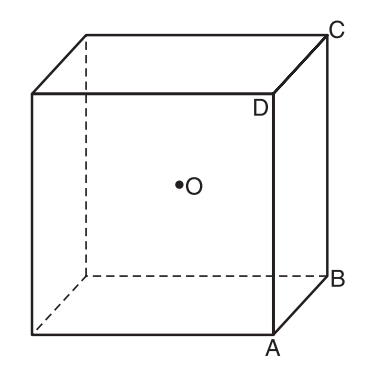
\includegraphics[scale=0.6]{qUFRS.png}
            \end{center} Se o volume do cubo é 1, o volume da pirâmide de base ABCD e vértice O é:
            
            \begin{enumerate}[label=(\alph*), noitemsep]
                \item ${1}/{2}$
                \item ${1}/{3}$
                \item ${1}/{4}$ 
                \item \vermelho{${1}/{6}$} %
                \item ${1}/{8}$
            \end{enumerate}
        
        \novaquestao{UFRJ 2000}
            Considerando um lustre de formato cônico com altura e raio da base igual a $0,25$ m, a distância do chão (H) em que se deve pendurá-lo para obter um lugar iluminado em forma de círculo com área de $25\pi m^{2}$, é de:

            \begin{center}
                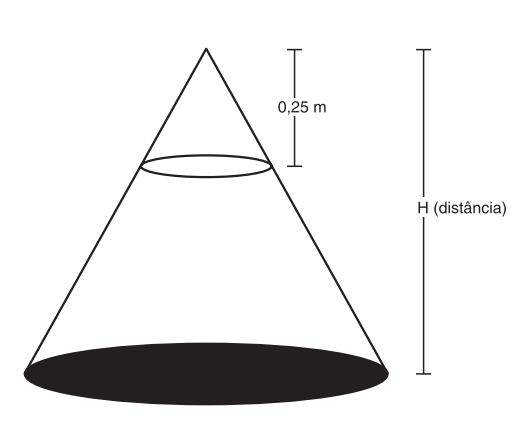
\includegraphics[scale=0.5]{UFRJ-CONE.png}
            \end{center} 
            
            \begin{enumerate}[label=(\alph*), noitemsep]
                \item 12 m
                \item 10 m
                \item 8 m
                \item 6 m
                \item \vermelho{5 m} %
            \end{enumerate}

        \novaquestao{Unifor-CE}
            Dois cones retos, $C_{1}$ e $C_{2}$, têm alturas iguais e raios da base de medidas $r_{1}$ cm e $r_{2}$ cm, respectivamente. Se $r_{1}=\dfrac{4}{5}r_{2}$, então a razão entre os volumes de $C_{1}$ e $C_{2}$, nessa ordem, é:

            \begin{enumerate}[label=(\alph*), noitemsep]
                \item \vermelho{${16}/{25}$} %
                \item ${18}/{25}$
                \item ${4}/{5}$ 
                \item ${22}/{25}$
                \item ${24}/{25}$
            \end{enumerate}

        \novaquestao{CEFET-RJ}
            Considere um cone cujo volume vale $7\pi\ cm^{3}$, inscrito num cilindro, como mostra a figura. A diferença entre os volumes do cilindro e do cone vale:

            \begin{center}
                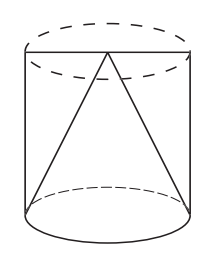
\includegraphics[scale=0.5]{cefet-rj-cone.png}
            \end{center}
            
            \begin{enumerate}[label=(\alph*), noitemsep]
                \item $\dfrac{7\pi}{3}\ cm^{3}$ \\
                \item $\dfrac{7\pi}{2}\ cm^{3}$ \\
                \item $7\pi\ cm^{3}$ 
                \item \vermelho{$14\pi\ cm^{3}$} % 
                \item $21\pi\ cm^{3}$ 
            \end{enumerate}

        \novaquestao{UFRGS 2001}
            A figura abaixo representa a planificação de uma pirâmide de base quadrada com AB = 6 cm, sendo ADV triângulo equilátero.

            \begin{center}
                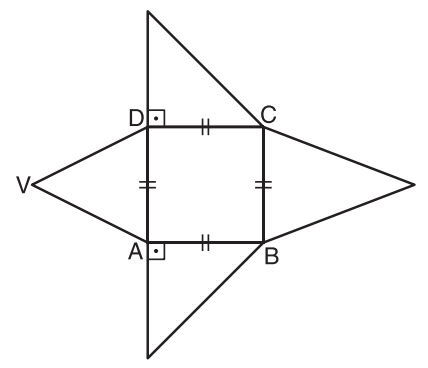
\includegraphics[scale=0.5]{ufrs-piramide.png}
            \end{center} O volume da pirâmide, em $cm^{3}$, é:
            
            \begin{enumerate}[label=(\alph*), noitemsep]
                \item $12\sqrt{3}$
                \item $27\sqrt{3}$
                \item \vermelho{$36\sqrt{3}$} 
                \item $72\sqrt{3}$
                \item $108\sqrt{3}$
            \end{enumerate}

        \novaquestao{UFPE}
            Na figura abaixo o cubo de aresta medindo 6 está dividido em pirâmides congruentes de bases quadradas e com vértices no centro do cubo. Qual o volume de cada pirâmide?

            \begin{center}
                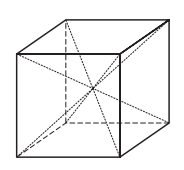
\includegraphics[scale=0.5]{ufpe-cubo.png}
            \end{center} 
            
            \begin{enumerate}[label=(\alph*), noitemsep]
                \item \vermelho{36}
                \item 48
                \item 54
                \item 64
                \item 72
            \end{enumerate}
        
            
    \end{multicols}
    
\end{document}